\documentclass[spanish,letterpaper,oneside]{article}

% Datos del documento
\def\documenttitle {Siete habilidades para el aprendizaje de las matemáticas}
\def\documentsubtitle {Fundamentos para la enseñanza y el aprendizaje I}
\def\documentsubject {Actividad 5 · Mapa mental y fundamentación docente}
\def\documentauthor {Mtro. Martín Jonathan de la Cruz Muñoz}
\def\coursename {Fundamentos para la enseñanza y el aprendizaje I}
\def\coursecode {MAEM}

% Identidad institucional
\def\universityname {Instituto de Investigación, Innovación y Estudios de Posgrado para la Educación del Estado de Nuevo León}
\def\universityfaculty {Maestría en Aprendizaje y Enseñanza de las Matemáticas}
\def\universitydepartment {Fundamentos para la enseñanza y el aprendizaje I}
\def\universitydepartmentimage {img/iiiepe/marca-iiiepe.png}
\def\universitydepartmentimagecfg {height=1.75cm}
\def\universitylocation {Monterrey, Nuevo León}
\def\studentfullname {Mtro. Martín Jonathan de la Cruz Muñoz}
\def\studentid {00874}
\def\studentemail {martin.delacruz@campus.iiiepe.edu.mx}
\def\programperiod {1er tetramestre, marzo--julio de 2026}
\def\programmodality {Modalidad presencial}
\def\programshort {MAEM}

\def\authortable {
  \begin{tabular}{ll}
    \textbf{Alumno:} & \studentfullname \\
    Matrícula: & \studentid \\
    Correo institucional: & \studentemail \\
    Unidad: & \coursename \\
    Programa: & \programshort \\
    Periodo: & \programperiod \\
    & \\
    \multicolumn{2}{l}{Fecha de realización: 13 de octubre de 2026} \\
    \multicolumn{2}{l}{\universitylocation}
  \end{tabular}
}

\input{template}

\usepackage{helvet}
\renewcommand{\familydefault}{\sfdefault}
\usepackage{array}
\usepackage{longtable}
\usepackage{pdflscape}
\usepackage{tikz}
\usepackage[most]{tcolorbox}
\usetikzlibrary{arrows.meta,positioning,calc,fit,backgrounds}

\definecolor{iiiepeNavy}{HTML}{163B5C}
\definecolor{iiiepeBlue}{HTML}{1F6F9F}
\definecolor{iiiepeAqua}{HTML}{20B7A8}
\definecolor{iiiepeOrange}{HTML}{F28C28}
\definecolor{iiiepePaper}{HTML}{F6F8F7}
\definecolor{iiiepeInk}{HTML}{1E2A32}
\def\portraittitlecolor {iiiepeNavy}
\setcitestyle{authoryear,open={(},close={)}}

\newcommand{\insertcoverwatermark}{%
  \AddToShipoutPictureBG*{%
    \begin{tikzpicture}[remember picture,overlay]
      \node[opacity=.09,inner sep=0pt] at (current page.center)
      {\includegraphics[width=.58\paperwidth]{img/iiiepe/logo-puntos.png}};
    \end{tikzpicture}%
  }%
}

\newtcolorbox{reportelecturabox}[1][]{%
  enhanced,breakable,
  colback=iiiepePaper,colframe=iiiepeNavy,
  boxrule=1pt,leftrule=4pt,arc=2pt,
  left=8pt,right=8pt,top=6pt,bottom=6pt,
  before skip=6pt,after skip=10pt,
  fonttitle=\bfseries\color{white},coltitle=white,
  colbacktitle=iiiepeNavy,
  attach boxed title to top left={xshift=8pt,yshift=-2pt},
  boxed title style={colback=iiiepeNavy,colframe=iiiepeNavy,arc=1pt},
  title={Reporte de lectura},#1}

\newtcolorbox{fichalecturabox}[1][]{%
  enhanced,breakable,
  colback=iiiepeAqua!7,colframe=iiiepeAqua!70!iiiepeNavy,
  boxrule=.6pt,arc=1pt,
  left=7pt,right=7pt,top=4pt,bottom=4pt,
  fontupper=\small,before upper={\setstretch{1.0}},
  fonttitle=\bfseries\color{iiiepeNavy},coltitle=iiiepeNavy,
  colbacktitle=iiiepeAqua!7,
  title={Ficha de la lectura},#1}



\usepackage{tabularx,colortbl,pgfplots,enumitem,needspace}\pgfplotsset{compat=1.18}\definecolor{iiiepePale}{HTML}{EEF5F8}
\setlength{\parskip}{5pt}\setlength{\parindent}{0pt}
\begin{document}\insertcoverwatermark\templatePortrait\templatePagecfg\templateFinalcfg\fancyfoot{}\fancyfoot[L]{\scriptsize IIIEPE · MAEM}\fancyfoot[C]{\scriptsize\thepage}\fancyfoot[R]{\scriptsize Actividad 5}\setstretch{1.3}\raggedbottom
\section{Habilidades para comprender y actuar}
Las siete habilidades presentadas por Wagner en la lectura de la plataforma vinculan pensamiento, colaboración, iniciativa, comunicación e interpretación de información. Su desarrollo exige tareas que permitan tomar decisiones, explicar razones y revisar propuestas. En mi contexto de CONALEP, CECyTE e ingenierías, propongo integrarlas en un problema de calibración, conservando atención a la persona y a sus condiciones de participación.
\section{Mapa mental}
\begin{center}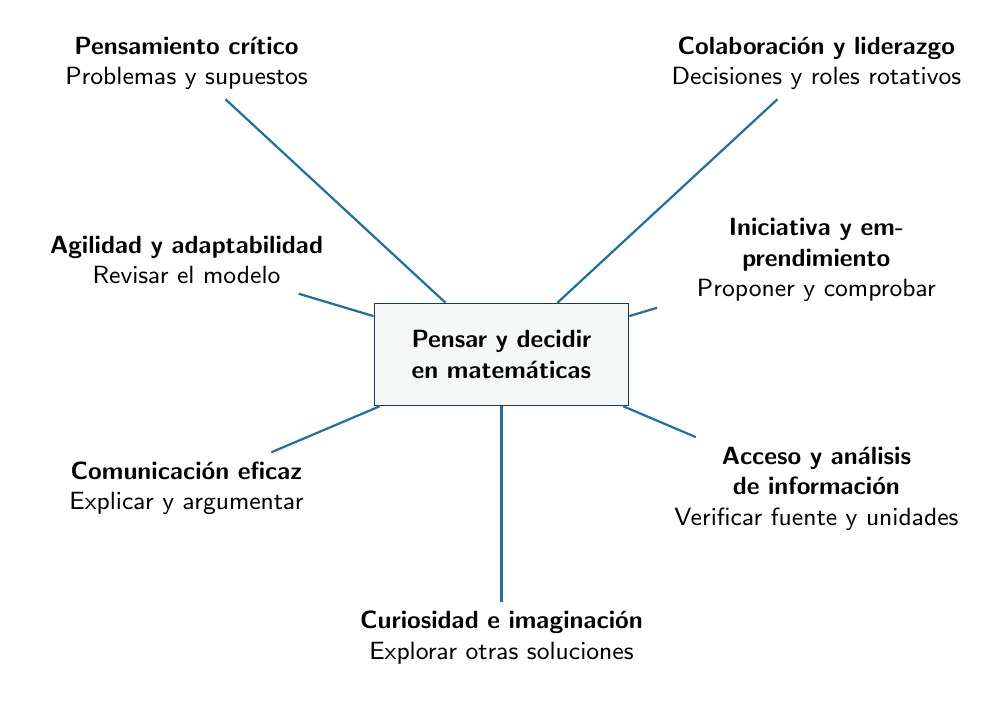
\begin{tikzpicture}[every node/.style={font=\small,align=center},edge/.style={thick,iiiepeBlue}]
\node[draw=iiiepeNavy,fill=iiiepePaper,text width=3cm,minimum height=1.3cm] (c) at (0,0){\textbf{Pensar y decidir\\en matemáticas}};
\node[text width=3.8cm] (a) at (-4,3.7){\textbf{Pensamiento crítico}\\Problemas y supuestos};
\node[text width=3.8cm] (b) at (4,3.7){\textbf{Colaboración y liderazgo}\\Decisiones y roles rotativos};
\node[text width=3.8cm] (d) at (-4,1.2){\textbf{Agilidad y adaptabilidad}\\Revisar el modelo};
\node[text width=3.8cm] (e) at (4,1.2){\textbf{Iniciativa y emprendimiento}\\Proponer y comprobar};
\node[text width=3.8cm] (f) at (-4,-1.7){\textbf{Comunicación eficaz}\\Explicar y argumentar};
\node[text width=3.8cm] (g) at (4,-1.7){\textbf{Acceso y análisis de información}\\Verificar fuente y unidades};
\node[text width=4cm] (h) at (0,-3.6){\textbf{Curiosidad e imaginación}\\Explorar otras soluciones};
\foreach \n in {a,b,d,e,f,g,h}\draw[edge] (c)--(\n);
\end{tikzpicture}\end{center}
\section{Cómo propongo promoverlas en matemáticas}
\subsection{Pensamiento crítico y resolución de problemas}
Plantearía si un sensor mantiene una relación proporcional entre lectura y referencia. El estudiante debe distinguir cociente constante de una relación con desplazamiento inicial, justificar el modelo y examinar un dato discrepante. La evidencia es una explicación que conecte tabla, gráfica y ecuación; acertar un valor aislado no basta.
\subsection{Colaboración y liderazgo}
Organizaría equipos con roles de medición, registro, cálculo y explicación, que roten. Cada integrante tendría que explicar una decisión compartida. El liderazgo se valoraría por facilitar participación y acuerdos sustentados, no por monopolizar la herramienta o imponer una respuesta.
\subsection{Agilidad y adaptabilidad}
Introduciría una condición nueva, como un cambio de escala o una lectura con sesgo, para que revisen el modelo. Adaptarse no significa modificar datos para obtener el resultado esperado; exige reconocer qué supuesto dejó de cumplirse y justificar una corrección.
\subsection{Iniciativa y espíritu empresarial}
Invitaría a proponer una mejora de bajo costo al procedimiento de medición, comparando recursos y beneficio esperado. La iniciativa debe incluir prueba y responsabilidad, no solo una idea atractiva. El criterio sería explicar por qué la propuesta es viable y qué evidencia permitiría revisarla.
\subsection{Comunicación oral y escrita eficaz}
Pediría un informe breve con problema, procedimiento, representación y conclusión, seguido de una explicación oral. El público debe comprender qué se calculó, con qué unidades y bajo qué condiciones. Una devolución entre pares revisaría si la conclusión se sostiene en los datos.
\subsection{Acceso a la información y análisis}
Compararía un manual, una lectura académica y una página sin autor identificable. Los estudiantes revisarían procedencia, fecha, unidades y ámbito de aplicación. Encontrar una fórmula no permite usarla sin comprobar si representa el fenómeno y las condiciones del problema.
\subsection{Curiosidad e imaginación}
Solicitaría dos estrategias para interpretar o resolver el problema: gráfica y algebraica, por ejemplo. La imaginación no se limita a decorar el producto; consiste en explorar relaciones y formular preguntas nuevas. Las alternativas se compararían por claridad, validez y límites.
\section{Un diseño matemático que hace visibles las habilidades}
Propongo estudiar la temperatura de un proceso didáctico mediante el modelo $T(t)=20+3t$, con $t$ en minutos y $T$ en grados Celsius, durante un intervalo definido. A los ocho minutos, $T(8)=44$; para alcanzar 50, $20+3t=50$ conduce a $t=10$. El modelo es ilustrativo y no representa la dinámica de un equipo industrial real.
El pensamiento crítico aparece al preguntar si el crecimiento puede mantenerse indefinidamente; la colaboración, al distribuir y revisar representaciones; la adaptabilidad, al incorporar un cambio de pendiente; la iniciativa, al proponer una prueba; la comunicación, al explicar la ecuación; el análisis de información, al revisar procedencia y unidades; y la curiosidad, al comparar modelos alternativos. La habilidad se reconoce en una acción vinculada con el contenido, no en una etiqueta agregada a la planeación.
Wagner (s. f.) permite examinar la distancia entre memorizar vocabulario y utilizarlo para resolver problemas. En mi contexto, el rigor técnico exige que el estudiante justifique una hipótesis; la perspectiva humanista exige condiciones para que todos puedan formularla y revisarla. El ejemplo anterior muestra cómo diseñaría esa integración y permite distinguirla de los resultados reales que habría que documentar al aplicarla.

{\small\setstretch{1.1}\renewcommand{\arraystretch}{1.25}
\begin{longtable}{|>{\raggedright\arraybackslash}p{\dimexpr0.32\linewidth-2\tabcolsep-2\arrayrulewidth\relax}|>{\raggedright\arraybackslash}p{\dimexpr0.68\linewidth-2\tabcolsep-2\arrayrulewidth\relax}|}\hline
\rowcolor{iiiepePale} \textbf{Indicador} & \textbf{Evidencia que se solicitaría} \\\hline
\endfirsthead
\hline
\rowcolor{iiiepePale} \textbf{Indicador} & \textbf{Evidencia que se solicitaría} \\\hline
\endhead
Argumentación & Explica la pendiente 3 y el valor inicial 20 con unidades. \\\hline
Transferencia & Resuelve un modelo con otra pendiente y compara el tiempo. \\\hline
Comunicación & Presenta una tabla y una conclusión que no exceda el intervalo del modelo. \\\hline
Colaboración y revisión & Explica una aportación propia y una corrección basada en una devolución. \\\hline
\end{longtable}}

\section{Fundamentación y postura docente}
La lectura de Wagner (s. f.) permite cuestionar tareas que exigen recordar información sin utilizarla. Mi interpretación es que las habilidades deben desarrollarse dentro del contenido: argumentar un modelo requiere conocimiento matemático, y colaborar requiere una tarea que necesite escuchar y contrastar. No sustituiría el contenido por habilidades generales ni daría por logrado un aprendizaje solo por trabajar en equipo.
Mi transición hacia una enseñanza humanista implica que el rigor técnico sirva para comprender y decidir, con espacios de participación y revisión. Evaluaría una primera explicación y otra posterior a la devolución. No afirmo que estas propuestas ya hayan generado resultados; establezco un diseño que puede aplicarse y analizarse con evidencia.

\needspace{5\baselineskip}\section*{Referencias}
{\setstretch{1.15}\setlength{\parskip}{6pt}
\par\hangindent=1.27cm\hangafter=1  Scott, C. L. (2015b). \textit{El futuro del aprendizaje 2: ¿Qué tipo de aprendizaje se necesita en el siglo XXI?} (Investigación y prospectiva en educación, 14). UNESCO.
\par\hangindent=1.27cm\hangafter=1  Secretaría de Educación Pública. (2022). \textit{Plan de Estudio para la educación preescolar, primaria y secundaria}. SEP.
\par\hangindent=1.27cm\hangafter=1  Wagner, T. (s. f.). \textit{Las siete habilidades de supervivencia para la profesión, el colegio y la ciudadanía}. Lectura proporcionada en EVA.
}

\end{document}
